\chapter{Arquitetura}

\section{Interação entre as partes}
Um utilizador apenas interage com o servidor regional onde este está registado. O servidor regional comunica-se com o utilizador e com o servidor central. O servidor central apenas interage com os servidores regionais.

\begin{figure}[h]
	\makebox[\textwidth][c]{
		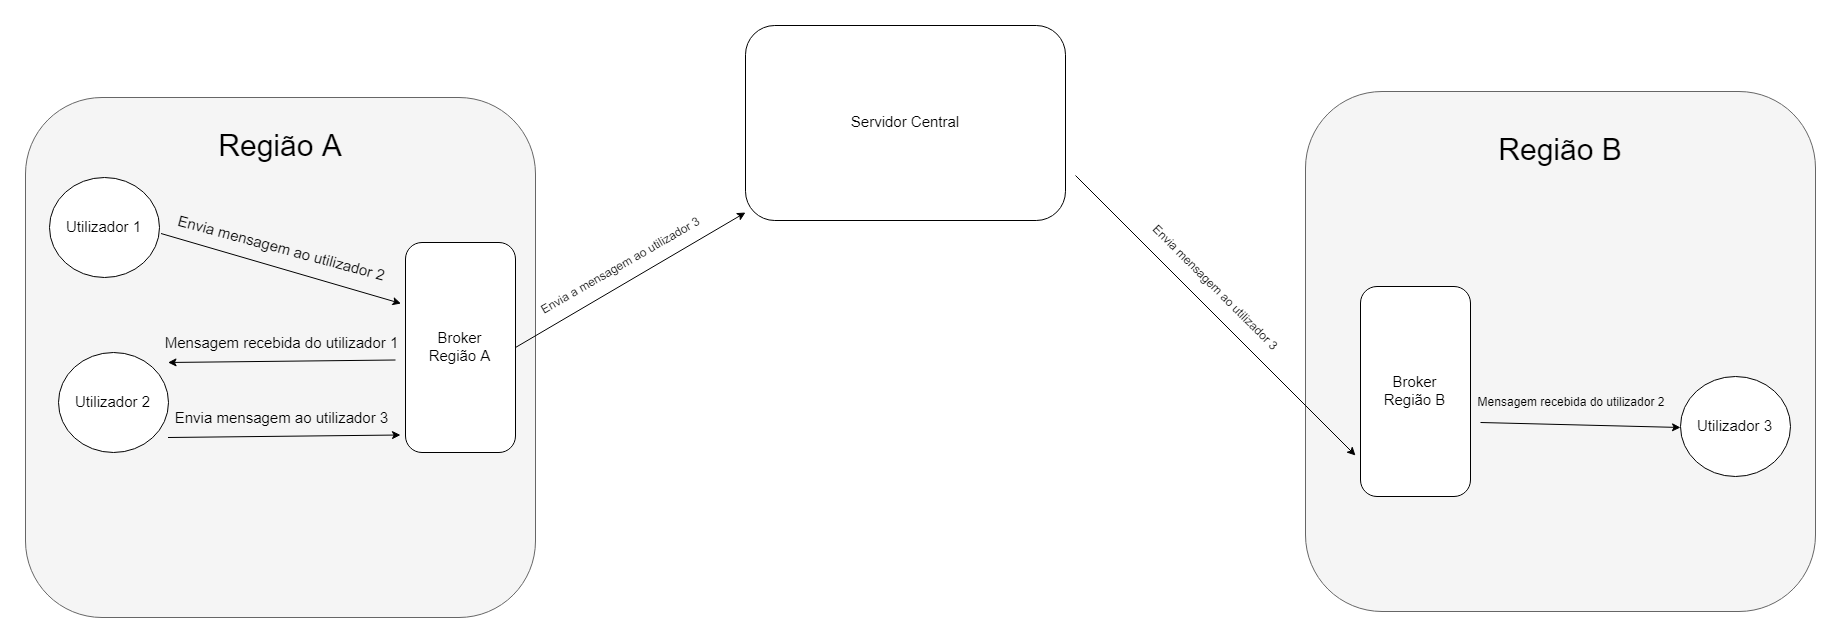
\includegraphics[width=1.3\textwidth]{./figures/diagram}
	}
\end{figure}

O utilizador é cliente do servidor regional. O servidor regional é servidor do utilizador e cliente do servidor central. O servidor central é servidor do servidor regional.

\section{Funcionamento}

Para poder utilizar o sistema, o utilizador deve escolher em qual região pretende-se conectar. Estando este conectado, é possível usufruir das seguintes funcionalidades:
\begin{itemize}
	\item Enviar mensagens para o utilizador;
	\item Criar grupos;
	\item Enviar mensagens para um grupo;
	\item Trocar de região;
	\item Sair de uma região.
\end{itemize}

\subsection{Funcionamento entre utilizadores}
Para um utilizador enviar uma mensagem para outro utilizador da mesma região o processo ocorre apenas no servidor dessa região. Caso o utilizador deseje enviar uma mensagem para outro utilizador fora da sua região, o servidor da região irá comunicar-se com o servidor central dizendo para este tratar de enviar a mensagem para um determinado utilizador que o servidor regional não tem conhecimento. O servidor central irá enviar a mensagem a todos os servidores regionais que conhece e estes irão verificar se o utilizador encontra-se registado na respetiva região. Em caso afirmativo tratarão de enviar a mensagem para o utilizador pretendente. Em caso negativo, o servidor regional não comunica com nenhum utilizador.

\subsection{Funcionamento em grupo}
É possível ao utilizador criar grupos dentro de uma região e adicionar outros utilizadores quer estejam na mesma ou em diferentes regiões. A existência do grupo é replicada por todos os outros servidores regionais. Ao adicionar um utilizador de outra região, o servidor regional envia a informação ao servidor central, que por sua vez envia aos outros servidores regionais até que a região onde se encontra o utilizador receba a mensagem e o adiciona ao grupo. Aos utilizadores que pertençam a um grupo, estes têm permissão para adicionar outros utilizadores. Os utilizadores que pertencem a um grupo nunca podem sair desse grupo, só sairão quando o criador apagar o grupo.